\documentclass[border=5pt]{standalone}
%\usepackage{bera}
%\renewcommand{\familydefault}{\sfdefault}
\usepackage{tikz}
\usepackage{pgfbasepatterns}
\usepgflibrary{arrows}
\usepgflibrary{patterns}
\usepgflibrary{snakes}

\begin{document}

\pagestyle{empty} 
\begin{Large}
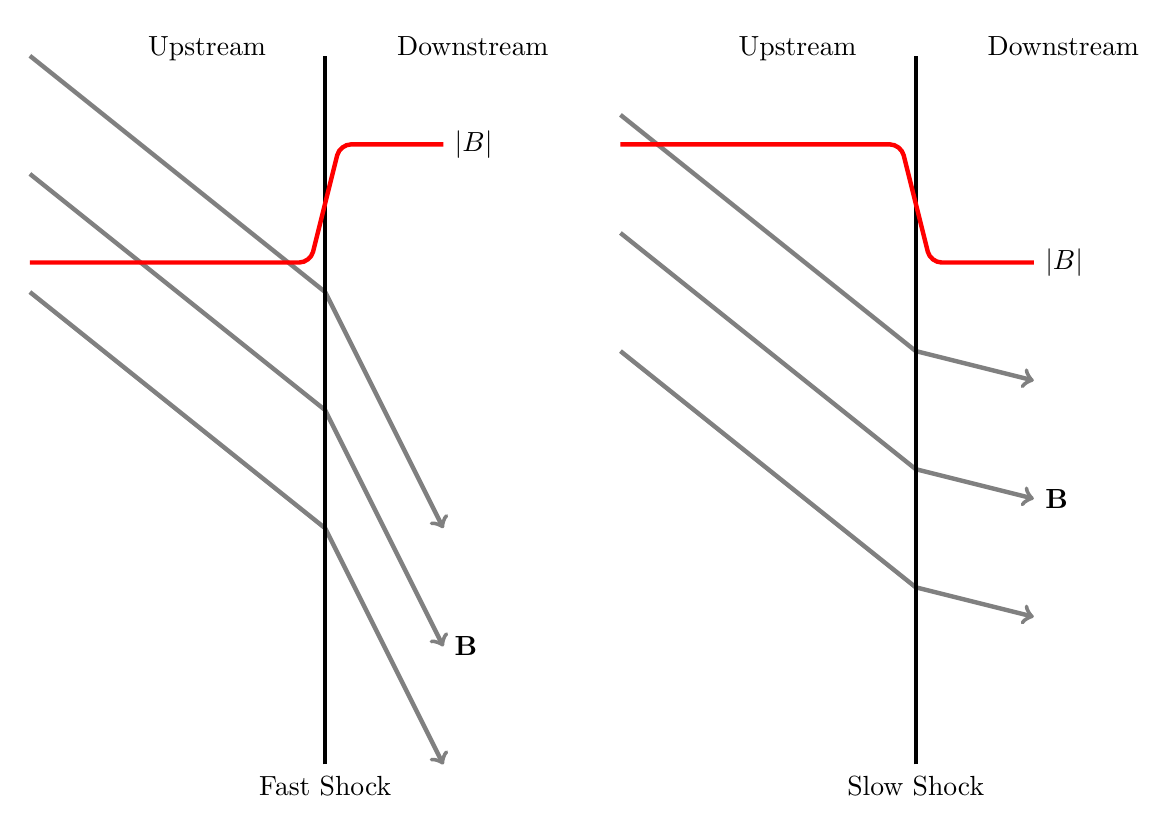
\begin{tikzpicture}[ultra thick]
\begin{scope}[scale=0.75]
  \begin{scope}[gray]
    \foreach \y in {0,2,4}
    {
    \draw (0,\y) -- +(-5,4);
    \draw[->] (0,\y) -- +(2,-4);
    }
  \end{scope}

  \draw (2,-2) node [right] {$\mathbf{B}$};

  \draw (0,-4) node [below] {Fast Shock} -- (0,8);
  \draw (-2,8) node [anchor=base] {Upstream};
  \draw (2.5,8) node [anchor=base] {Downstream};

  \draw [rounded corners,color=red,smooth] (-5, 4.5) -- (-0.25,4.5) -- (0.25,6.5) -- (2,6.5) node [right,black] {$|B|$};

	\begin{scope}[xshift=10cm]

  \begin{scope}[gray]
    \foreach \y in {-1,1,3}
    {
    \draw (0,\y) -- +(-5,4);
    \draw[->] (0,\y) -- +(2,-0.5);
    }
  \end{scope}

  \draw (2,0.5) node [right] {$\mathbf{B}$};

  \draw (0,-4) node [below] {Slow Shock} -- (0,8);
  \draw (-2,8) node [anchor=base] {Upstream};
  \draw (2.5,8) node [anchor=base] {Downstream};

  \draw [rounded corners,color=red,smooth] (-5, 6.5) -- (-0.25,6.5) -- (0.25,4.5) -- (2,4.5) node [right,black] {$|B|$};

	\end{scope}
\end{scope}
\end{tikzpicture}
\end{Large}
\end{document}

%%% Local Variables: 
%%% mode: latex
%%% TeX-master: t
%%% TeX-PDF-mode: t
%%% End: 
